\subsection{Implementation}
We implemented the SVM using quadratic programming. We used the solver from the \texttt{cvxopt\footnote{https://cvxopt.org/}} library to solve the optimization problem. A SVM is based on a percentron, but instead oof chosing any separating hyperplane, we choose the one with the largest margin. This can be expressed as a quadratic program in the following form.
\begin{align*}
	\min&&\, \frac{1}{2}\lVert w \rVert&&  \\
	\text{s.t.}&&\, (\omega^tx_i+w_0)t_i && 1 \leq i \leq N.
\end{align*}
Instead of solving this directly we search the dual problem of this solution. This problem is given by following quadratic program.
\begin{align*}
	\max&& - \frac{1}{2} \sum\limits_{i=1}^N \sum\limits_{j=1}^N&\alpha_i\alpha_jt_it_j(x_i^tx_j) +  \sum\limits_{i=1}^N \alpha_i &\\
	\text{s.t.}&& \sum\limits_{i=1}^N\ \alpha_i t_i &= 0& \\
	&&\alpha_i&\geq0& 1\leq i \leq N
\end{align*}
We see sone advantages of this formulation. There is an equality instead of an inequality and we also see that we only have to calculate an inner product, this will be useful when we use the kernel trick.

The solver from \texttt{cvxopt} assumes that the input has the form
\begin{align*}
	\min&& \frac{1}{2} x^tPx &+ q^t&\\
	\text{s.t.}&&Gx&\leq h& \\
	&&Ax&=b& 
\end{align*}
With $x=\bm{\alpha}$ we get following matrices and vectors for our problem. $P=\sum\limits_{i=1}^N \sum\limits_{j=1}^Nt_it_j(x_i^tx_j)$, $q=\bm{1}$, 
$G=-\mathbb{I}$, $h=\bm{0}$, $A=t^t$ and $b=0$.

Once we have solved the problem, we get the (dual) solution $\bm{\alpha}$. The $x_i$ for which $\alpha_i>0$ are called support vectors. From this we can calculate $\omega$ and $\omega_0$. We pick the support vector with the largest $\alpha_i$, say with $i = i_{\max}$, and then:
\[
	\omega = \sum\limits_{i=1}^N\alpha_i t_i \bm{x_i}
\]
and 
\[
	\omega_0 = t_{i_{\max}} - \omega^t\bm{x_{i_{\max}}}.
\]
In the sum to calculate $\omega$ most $\alpha_i$ are $0$, thus we only need to consider suport vectors to calculate $\omega$.

With this we can also calculate the discriminant function and we don't need to calculate $\omega$ as it only depends on $\alpha_i$, $t_i$ and $x_i$. This gives us for new data points:
\[
	d(x) = \omega_0 + \sum_{i=0}^N\alpha_it_i(x^tx_i),
\]
where we again only need to sum over the support vectors.
\subsection{Validation}

We used a synthetic generated set to test our implementation. We used the make blobs function of \texttt{scikit-learn\footnote{https://scikit-learn.org}} to generate the datset. We used two clusters with centers at $(1,1)$ and $(-1,-1)$ and standard deviation of $0.9$. For 200 data points and seed $=6$ we got a linearly seperable dataset. We then applied to trained SVM to the same clusters, but with 400 data points and different seed. The optimal parameters would be $\omega_0 = 0$ and $\omega = \lambda (1,1)$. We got following results. The two datesets with the decision boundry and margins are shown in figure \ref{task1::svm}. We see that one outlier was classified wrongly in the test set and naturally no in the training set, as the set is linearly separable.
\begin{itemize}
	\item $\omega_0 = 0.037$
	\item $\omega = (0.9345, 0.9475)$
\end{itemize}
\begin{figure}
	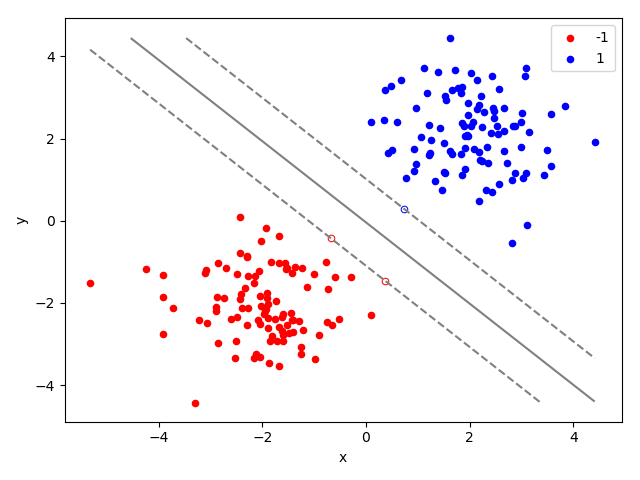
\includegraphics[width=0.5\textwidth]{task1_train}
	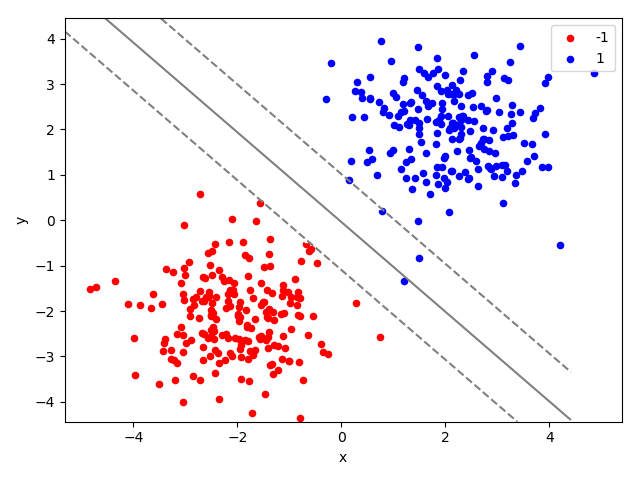
\includegraphics[width=0.5\textwidth]{task1_test}
	\caption{Trainng and testing of a SVM. Left ist training and right is testing.}
	\label{task1::svm}
\end{figure}

We see that if we used the training set to train the SVM the result would be a worse decision boundry. For this we will introduce slack variables in the next task. The new formulation will also be able to handle sets that are not linearly separable.
